% Do not remove the next line
% Synchronized to r45459

\section{Le filtrage de paquets}
\configlabel{PF\_NEW\_CONFIG}{PFNEWCONFIG}

\newcommand{\fwaction}[1]{{\small\textsf{#1}}}
\newcommand{\fwchain}[1]{\texttt{#1}}
\newcommand{\fwtable}[1]{\textsc{#1}}
\newcommand{\fwmatch}[1]{\texttt{#1}}
\newcommand{\fwpktstate}[1]{\texttt{#1}}
\newcommand{\fwloglevel}[1]{\texttt{#1}}
\newcommand{\protocol}[1]{\texttt{#1}}
\newcommand{\host}[1]{\texttt{#1}}
\newcommand{\package}[1]{\texttt{#1}}

  Le Kernel de Linux utilisé par fli4l met à disposition un filtrage de paquets.
  A l'aide de ce filtrage de paquets, on contrôle les flux qui communiquent avec
  le routeur et au de là de celui-ci. Par ailleurs, vous pouvez réaliser des
  dispositifs comme la redirection de port (redirige les paquets réçus par le
  routeur et les transmettre à un ordinateur du réseau interne) et le masquage
  (en anglais masquerading. Les paquets provenant d'un ordinateur du réseau
  interne derrière le routeur sont modifiés, de telle sorte que ces paquets
  semblent provenir du routeur lui-même).

  La structure du filtrage de paquets est indiquée sur le schéma
  \ref{fig:netfilter}. Les paquets qui entrent par l'interface réseau, parcourent
  la chaîne \fwchain{PREROUTING} (en anglais "chain"). le routeur qui reçoit les
  paquets sont manipulés, ils sont ensuites renvoyés vers un autre ordinateur en
  utilisant l'adresse et le port de destination. Si les paquets sont adressés
  au routeur, ils parcourent la chaîne \fwchain{INPUT}, sinon ils parcourent
  la chaîne \fwchain{FORWARD}. Les deux chaînes examinent si les paquets sont
  autosisés à passer. S'il sont acceptés, les paquets sont envoyés sur le
  processus cible locale ou vers la chaîne \fwchain{POSTROUTING} (ici le
  masquage de paquets a lieu) ensuite les paquets passent par l'interface réseau
  et peuvent atteindre leur destination. Les paquets générés localement sont
  filtrés dans la chaîne \fwchain{OUTPUT} et enfin (en cas de succès) les paquets
  sont envoyés dans la chaîne \fwchain{POSTROUTING} et sont également transmis
  en passant par l'interface réseau.

  \begin{figure}[htbp]
    \centering
    \includegraphics[width=\columnwidth]{netfilter}
    \caption{Structure du Filtrage de paquets}
    \label{fig:netfilter}
  \end{figure}

  La configuration les chaînes de filtrage de paquets, peut être paramétré
  séparément. En plus il y a une liste pertinente pour chaque chaîne importante,
  c.-à-d. pour la chaîne \fwchain{INPUT} vous avez (\var{PF\_INPUT\_\%}), pour
  la chaîne \fwchain{FORWARD} vous avez (\var{PF\_FORWARD\_\%}), pour la chaîne
  \fwchain{PREROUTING} vous avez (\var{PF\_PREROUTING\_\%}) dans laquelle vous
  effectuez la redirection de ports et pour la chaîne \fwchain{POSTROUTING} vous
  avez (\var{PF\_POSTROUTING\_\%}) dans laquelle vous exécutez le masquage
  de paquets.

  Le paramètrage de la liste se compose principalement d'une action (voir
  ci-dessous), qui peut être limitée par des conditions supplémentaires. Ces
  conditions portent sur les propriétés du paquet. Un paquet contient des
  informations sur son origine (la source quel ordinateur a envoyé le paquet),
  sa cible (à quel ordinateur et quelle application le paquet doit aller), etc.
  les conditions du paquet peuvent être basées sur les propriétés suivantes~:

\begin{itemize}
  \item La source (adresse source, port source, ou les deux)
  \item La destination (adresse de destination, le port de destination, ou les deux)
  \item Le protocole
  \item L'interface sur laquelle le paquet entre ou sort
  \item L'adresse MAC de l'ordinateur qui a envoyé le paquet
  \item L'état du paquet ou du lien dont le paquet fait partie
\end{itemize}

  Si un paquet entre, les enregistrements ou les règles générées sont récupérées
  de haut en bas, la première action est exécutée et toutes les conditions. Si
  aucune des règles ne s'applique, l'action par défaut est exécutée, vous pouvez
  spécifier des règles pour (presque) toutes les tables.

  Un enregistrement a la forme suivant, vous devez faire attention que toutes
  les restrictions sont optionnelles~:

\begin{example}
\begin{verbatim}
    restriction{0,} [[source] [destination]] action [BIDIRECTIONAL|LOG|NOLOG]
\end{verbatim}
\end{example}

  Sur les points qui conserne le réseau vous devez spécifier une adresse IP
  ou un hôte. vous pouvez aussi utiliser les variables \var{IP\_NET\_\%},
  \var{IP\_NET\_\%\_IPADDR} ou un \host{@non\_d'hôte} via les variables \var{HOST\_\%}.
  Si la variable \var{OPT\_DNS} est activées, vous pouvez référencer un nom
  externe au réseau local via \host{@fqdn}, mais vous ne devez \emph{pas}
  récupérer le nom dans la variable \var{HOST\_\%}. Cela est particulièrement
  utile, quand il s'agit d'hôtes externes, et qu'ils possèdent en plus des
  adresses IP dynamique (ou changeante).

\marklabel{sec:fwrules_actions}{\subsection{Action pour le filtrage de paquets}}

Les actions peuvent être les suivants~:
\begin{center}
    \begin{longtable}{|l|l|p{0.5\textwidth}|}
        \hline
        \multicolumn{1}{|l}{\textbf{Action}} &
        \multicolumn{1}{|l}{\textbf{Chaîne(n)}} &
        \multicolumn{1}{|l|}{\textbf{Importance}} \\
        \hline
        \endhead
        \hline
        \endfoot
        \endlastfoot
        \fwaction{ACCEPT}       & Tous
                                & Accepte le paquet
                                \\
        \hline
        \fwaction{DROP}         &
                                \begin{tabular}[t]{@{}l@{}}
                                    \fwchain{INPUT} \\
                                    \fwchain{FORWARD} \\
                                    \fwchain{OUTPUT}
                                \end{tabular}
                                & Le paquet est rejeté (l'expéditeur ne recevera
                                pas de réponse et aucun message ne lui reviendra).
                                \\
        \hline
        \fwaction{REJECT}       &
                                \begin{tabular}[t]{@{}l@{}}
                                    \fwchain{INPUT} \\
                                    \fwchain{FORWARD} \\
                                    \fwchain{OUTPUT}
                                \end{tabular}
                                & Le paquet est rejeté mais (l'expéditeur
                                recevera un message d'erreur).
                                \\
        \hline
        \fwaction{LOG}          & Tous
                                & Le paquet est enregistré et continu sur la règle
                                suivante. Vous pouvez utiliser un préfixe pour
                                différencier les entrées dans le fichier journal,
                                en spécifiant \fwaction{LOG:log-prefix}. Le préfix
								peut avoir une longueur de 28 caractères et peut
								contenir des lettres, des chiffres, le trait d'union
								(\texttt{-}) et le tiret bas (\texttt{\_}).
                                \\
        \hline
        \fwaction{MASQUERADE}   & \fwchain{POSTROUTING}
                                & Le paquet est masqué~: l'adresse source du
                                paquet sera remplacement par la propre adresse de
                                l'interface, adresse que vous lui aviez attribuée,
                                assurez-vous que la réponse est correctement
                                transmise à l'ordinateur source.
                                \\
        \hline
        \fwaction{SNAT}         & \fwchain{POSTROUTING}
                                & L'adresse et le port source du paquet seront
                                remplacement, la variable sera paramètrée comme
                                ceci \fwaction{SNAT} spécifier l'adresse (considéré
                                que tous les paquets appartiennent à cette connexion).
                                \\
        \hline
        \fwaction{DNAT}         & \fwchain{PREROUTING}
                                & L'adresse et le port de destination seront
                                remplacement, la variable sera paramètrée comme
                                ceci \fwaction{DNAT} spécifier l'adresse (considéré
                                que tous les paquets appartiennent à cette connexion).
                                \\
        \hline
        \fwaction{REDIRECT}     &
                                \begin{tabular}[t]{@{}l@{}}
                                    \fwchain{PREROUTING} \\
                                    \fwchain{OUTPUT}
                                \end{tabular}
                                & Le port de destination du paquet sera remplacer,
                                la variable sera paramètrée comme ceci \fwaction{REDIRECT}
                                spécifier le port, le paquet généré sera mappé au 
                                niveau local (considéré que tous les paquets
                                appartiennent à cette connexion).
                                \\
        \hline
        \fwaction{NETMAP}       &
                                \begin{tabular}[t]{@{}l@{}}
                                    \fwchain{PREROUTING} \\
                                    \fwchain{POSTROUTING}
                                \end{tabular}
                                & Crée une image de l'adresse cible ou de la source
                                du paquet, la variable sera paramètrée comme ceci
                                \fwaction{NETMAP} spécifier l'adresse du domaine,
                                les ports restent inchangés (considéré que tous 
                                les paquets appartiennent à cette connexion, dans
                                la chaîne \fwchain{PREROUTING} l'adresse de
                                destination sera modifiée et dans la chaîne
                                \fwchain{POSTROUTING} c'est l'adresse de source
                                qui sera modifiée).
                                \\
        \hline
        \caption{Action des règles du filtrage de paquets}\marklabel{fwrule:actions}{}
    \end{longtable}
\end{center}

On peut modifier le comportement de certaines de ces actions avec les
options suivant \fwaction{BIDIRECTIONAL}, \fwaction{LOG} ou \fwaction{NOLOG}.
L'option \fwaction{BIDIRECTIONAL} génère à nouveau la même règle, mais avec une
adresse source et destination inversée (un changement de port source et destination
et/ou un changement de l'interface réseau sortant si elle est spécifiée). Les
options \fwaction{LOG}/\fwaction{NOLOG} active ou n'active pas le fichier journal
pour cette règle.

\marklabel{sec:fwrules_limits}{\subsection{Restriction dans les règles}}

les restrictions peuvent être réalisés, elle sont indiquées dans ce chapitre
ci-dessous. Si vous ne voulez pas faire de restriction vous pouvez toujours
spécifier \fwmatch{any}, mais vous devez toujours indiquer quelque chose.
Les restrictions peuvent être spécifiées dans n'importe quel ordre, si le
préfixe est préposé. Cela s'applique à toutes les restrictions, sauf pour
spécifier une adresse source ou destination. Ceux-ci doivent toujours être
directement devant l'action, les autres restrictions doivent être faites avant.
Les restrictions peuvent également être annulés, en préposant tout simplement 
le symbole \fwmatch{!}

\subsubsection{Restriction de la source et de la destination}

Chaque paquet contient une source et une cible, respectivement sous la forme
multiplet d'adresse IP et de port. \footnote{Le port est disponible seulement
pour les paquets avec le protocole TCP et UDP.} Cette source ou cette cible
peut être utilisé pour une restriction. La spécification de la source ou de la
destination peut être faite comme ceci~:

\begin{center}
    \begin{longtable}{|l|p{0.5\textwidth}|}
        \hline
        \multicolumn{1}{|l}{\textbf{Expression}} &
        \multicolumn{1}{|l|}{\textbf{Importance}} \\
        \hline
        \endhead
        \hline
        \endfoot
        \endlastfoot
    \verb+ip+               & Une seule adresse IP\\
    \verb+network+          & Spécification du réseau sous la forme \verb+<ip>/<netmask>+ \\
    \verb+port[-port]+      & Port ou une plage de ports\\
    \verb+IP_NET_x_IPADDR+  & Adresse IP de l'interface \verb+x+ du routeur\\
    \verb+IP_NET_x+         & Sous-réseau \verb+x+ du routeur\\
    \verb+IP_ROUTE_x+       & Spécifier la route \verb+x+ du sous-réseau
      (Les routes par défaut ne peuvent pas être utilisés, elles seraient toutes
      \fwmatch{any}, et sont exclus par précaution)\\
    \verb+@name+            & Nom ou alias attribué, dans la variable HOST\_\%\_*
      l'adresse IP est utilisé au nom associée\\
    \verb+<ip ou réseau>:port[-port]+ & Hôte ou l'adresse du réseau de l'une des
    variantes ci-dessus, combiné à un port ou une plage de ports\\
        \hline
        \caption{Restrictions de la source et de destination dans les règles de filtrage de paquets}
    \end{longtable}
\end{center}

\noindent Cela pourrait par exemple, ressembler à ceci~: \verb+'192.168.6.2 any DROP'+

Si on regarde ces paramètres, le premier est la source, le second est considéré
comme la cible. Dans cet exemple, nous rejetons les paquets qui ont été envoyées
par l'ordinateur avec l'adresse IP 192.168.6.2 et peu importe sur quelle
destination ils sont adressés.

Si un seul paramètre est indiqué, on peut décider en fonction de la valeur, si
c'est la source ou si c'est la destination qui est concernée, la décision est
relativement simple~:
\begin{itemize}
  \item Si le port est paramétré, ce sera la cible qui est concernée.
  \item Sinon, ce sera la source qui est concernée.
\end{itemize}

Si nous voulons écrire plus brièvement l'exemple ci-dessus~:
\verb+'192.168.6.2 DROP'+. Aucun port n'est indiqué, donc l'IP de l'ordinateur
est la source (c'est lui qui envoie les paquets).

Si nous voulons communiquer avec le démon \protocol{ssh}, nous pouvons indiquer
\verb+'any any:22 ACCEPT'+ (les paquets seront acceptés depuis n'importe quel
ordinateur sur le Port 22 du \protocol{ssh} et n'importe quel ordinateur les
acceptera), vous pouvez indiquez aussi \verb+'22 ACCEPT'+ seul un port est indiqué,
nous pouvons dire que c'est la cible, les paquets seront dirigés sur le port 22.

Pour simplifier la quantité de règle à écrire, on peut utiliser l'action
\fwaction{BIDIRECTIONAL} elle indique que les communications se feront dans
les deux sens. Les règles sont paramétrées simplement avec l'IP source, l'IP
destination et le port ou avec les interfaces réseau, les échanges entre cet
deux réseaux reste le même.

Exemple~:
\medskip

\begin{example}
\noindent
{\footnotesize
 \begin{tabular}{@{}p{5cm}p{10cm}@{}}
    \verb+127.0.0.1 ACCEPT+             & La communication locale (Souce 127.0.0.1) est accepté \\
    \verb+any 192.168.12.1 DROP+        & Les paquets vers l'adresse IP 192.168.12.1 sont rejetés \\
    \verb+any 192.168.12.1 DROP LOG+    & Les paquets vers l'adresse IP 192.168.12.1 sont rejetés et sont également enregistrés \\
    \verb+any 192.168.12.1 DROP NOLOG+  & Les paquets vers l'adresse IP 192.168.12.1 sont rejetés, ne sont pas enregistrés \\
    \verb+22 ACCEPT+                    & Les paquets vers le port 22 (\protocol{ssh}) sont acceptés \\
    \verb+IP_NET_1_NET ACCEPT+          & Les paquets du sous-réseau de la première interface sont acceptés\\
    \verb+IP_NET_1_NET IP_NET_2_NET+    & La communication entre la première et la seconde\\
    \verb+  ACCEPT BIDIRECTIONAL+       & L'interface du sous-réseau est acceptée
 \end{tabular}
}
\end{example}

\subsubsection{Restriction des interfaces}

Une règle peut restreindre une interface sur laquelle les paquets arrivent et
sortent. Le format de restriction est le suivant~:
\fwmatch{if:}\emph{in}\fwmatch{:}\emph{out}

Dans la chaîne \fwchain{INPUT} on ne peut pas restreindre l'interface pour les
paquets sortant (les paquets ne sortiront plus). Dans la \fwchain{POSTROUTING}
on ne peut pas restreindre l'interface pour les paquets entrant, car l'information
n'est plus disponible à ce moment là. Vous pouvez restreindre une interface
uniquement dans la chaîne \fwchain{FORWARD} pour les deux conditions (entrant
et sortant).

Les valeurs suivantes sont possibles pour \emph{in} ou \emph{out}~:

\begin{itemize}
  \item \fwmatch{lo} (Interface de bouclage, communication locale sur le routeur)
  \item \verb+IP_NET_x_DEV+ 
  \item \fwmatch{pppoe} (Interface PPPoE, seulement si le \package{dsl} ou le
    \package{pppoe\_server} est activé)
  \item \fwmatch{any}
\end{itemize}

\subsubsection{Restriction du protocole}

Une règle peut restreindre le protocole donc le paquet appartient. Le format
est le suivant~:
\fwmatch{prot:}\emph{protocol} ou bien \fwmatch{prot:}\emph{icmp}\fwmatch{:}\emph{icmp-type}.
\emph{protocol} peut prendre les valeurs suivantes~:

\begin{itemize}
  \item \fwmatch{tcp}
  \item \fwmatch{udp}
  \item \fwmatch{gre} (Generic Routing Encapsulation)
  \item \fwmatch{icmp} (Vous pouvez spécifier un nom pour le type de filtrage
    ICMP (\fwmatch{echo-reply} ou \fwmatch{echo-request}, en gros
    \fwmatch{prot:icmp:echo-request}
  \item Valeur numérique du protocole ID (exemple 41 pour IPv6)
  \item \fwmatch{any}
\end{itemize}

Si vous voulez utiliser un numéro de port avec des protocoles différents dans une
règle, une telle restriction ne sera pas disponible, vous devez créer la règle en
\emph{deux fois}, une fois pour le \protocol{tcp} et une fois pour le \protocol{udp}.

\subsubsection{Restriction des adresses MAC}

Vous pouvez utiliser \fwmatch{mac:}\emph{mac-address} pour faire une restriction
de l'adresse MAC.

\subsubsection{Restriction sur l'état d'un paquet}

pour le filtrage de paquets fli4l utilise les informations de l'état des
connexions. Ces informations peuvent ensuite être utilisées pour filtrer les
paquets, pour une description plus détaillée sur l'état des connexions~:
\footnote{voir \altlink{http://www.sns.ias.edu/~jns/files/iptables_talk/x38.htm}}

\begin{center}
    \begin{longtable}{|l|p{0.7\textwidth}|}
        \hline
        \multicolumn{1}{|l}{\textbf{Etat}} &
        \multicolumn{1}{|l|}{\textbf{Importance}} \\
        \hline
        \endhead
        \hline
        \endfoot
        \endlastfoot
        \fwpktstate{INVALID}        & Le paquet n'appartient à aucune connexion
                                      connue.
                                    \\
        \fwpktstate{ESTABLISHED}    & Le paquet appartient à une connexion, le
                                      paquet a déjà circulé dans l'autre sens
                                      (réponse).
                                    \\
        \fwpktstate{NEW}            & Le paquet fait partie d'une nouvelle
                                      connexion ou appartient à une connexion,
                                      mais le paquet n'a pas encore circulé dans
                                      l'autre sens.
                                    \\
        \fwpktstate{RELATED}        & Le paquet fait partie d'une nouvelle connexion,
                                      mais il est déjà en relation avec une connexion
                                      existante (par ex. établissement d'une connexion
                                      avec le \protocol{ftp} pour le transfère de données).
                                    \\
        \hline
        \caption{Restriction des règles sur de filtrage de paquets}
    \end{longtable}
\end{center}

L'état du paquet est défini comme ceci~: \fwmatch{state:}\emph{état(s)}.
Si vous souhaitez spécifier plusieurs conditions, vous devez les sépare par
une virgule. Par exemple si vous voulez laisser passer seulement les paquets
qui appartiennent directement ou indirectement à une connexion vous paramétrez
\fwmatch{state:}\fwpktstate{ESTABLISHED,RELATED}, il est utile d'écrire
(ces états dans la chaîne \fwchain{INPUT} ou \fwchain{FORWARD}).

\subsubsection{Restriction sur les fréquences des actions}

Dans certaine circonstance, on aimerait limiter la fréquence des actions,
par ex. faire seulement une demande d'écho ICMP par seconde. Cela peut être
spécifié avec la commande limitation \fwmatch{limit}, le format sera le
suivant~: \fwmatch{limit:}\emph{fréquence:Burst}. La fréquence est en
\emph{n/unité de temps} qui sera donnée en (second, minute, hour, day), de plus
vous pouvez indiquer une suite d'événements successifs (Burst). Par exemple en
spécifiant \texttt{limit:3/minute:5} un maximum de trois événements par minute
sera permis et cinq événements successifs seront acceptés.

\marklabel{sec:templates}{\subsection{Utilisation d'un modèle pour le filtrage de paquets}}

Il est possible pour l'utilisateur de simplifier la configuration des données
de filtrage de paquets, en l'utilisant un modèle (Template) c'est un condensé
de règles prés enregistré qui est fréquemment utilisées. Il est ainsi possible de
combiner un certain nombre de règles de filtrage de paquets, dans cette
collection de règles un nom symbolique y est associé. Au lieu d'écrire directement
dans la variable le protocole et le numéros de port il suffit d'écrire le nom
symbolique, si vous voulez utiliser le protocole \protocol{ssh} dans une règle
il suffit d'écrire \fwmatch{tmpl:ssh}. Comment faut-il procéder avec le modèle
\protocol{ssh}, vous avez un exemple d'utilisation ci-dessous.

Si vous voulez atteindre votre routeur fli4l par Internet avec le \protocol{ssh}, vous
devez écrire dans la variable \var{PF\_INPUT\_\%} le nom du service correspondant
(ici \protocol{ssh}), précédée par \fwmatch{tmpl:} et l'action qui consiste à
appliquer ce service. Par exemple~:

\begin{example}
\begin{verbatim}
    PF_INPUT_2='tmpl:ssh ACCEPT'
\end{verbatim}
\end{example}

Voici comment utiliser \emph{tmpl:} pour appliquer une règle dans un modèle.
Vous donnez le nom du service après les ':', dans notre exemple \protocol{ssh}.
Enfin, vous pouvez spécifier quelle action doit être connecté au service.
Puisque vous voulez communiquer avec fli4l à partir d'Internet, nous autorisons
la connexion avec \fwaction{ACCEPT}. La limitation des adresses IP ou des réseaux
ne sont pas spécifiées, Avec le service \protocol{ssh} tous les réseaux et toutes
les interfaces sont accessibles. Vous pouvez utiliser en cas de besoin la
configuration habituelle du filtrage de paquets pour limiter l'accès au service
\protocol{ssh}.

Pour quels services des règles sont ils préparées (c.-à-d. le modèle existent),
vous pouvez trouver dans le fichier \verb+opt/etc/fwrules.tmpl/templates+ le
modèle de service prés configuré. Voir ci-dessous la liste (dans le tableau
\ref{tab:fwrules_tmpl}).

\begin{center}
  {\footnotesize
  \begin{longtable}{|lll|}
     \hline
     {\textbf{Modèle}} & {\textbf{Protocole}} & {\textbf{Port(s)}} \\
     \hline\hline
     \endhead
     \input{fwrules_tmpl_table.inc} \\
     \hline
     \caption{Modèles inclus dans fli4l de base}
     \label{tab:fwrules_tmpl}
  \end{longtable}}
\end{center}

La syntaxe pour cette forme de règles de filtrage de paquets est toujours

\begin{example}
\begin{verbatim}
    tmpl:<Nom du service> <Restriction> <Action souhaitée>
\end{verbatim}
\end{example}

Les \verb+<restrictions>+ permisent sont décrites dans dans la section
\ref{sec:fwrules_limits}. Les valeurs possibles pour les \verb+<actions souhaitées>+
sont énumérées et décrites dans la section \ref{sec:fwrules_actions}

Voici quelques exemples pour illustrer la démarche. Nous allons d'abord
utiliser \var{PF\_PREROUTING}~:

\begin{example}
\begin{verbatim}
    PF_PREROUTING_N='2'
    PF_PREROUTING_1='tmpl:xbl dynamic DNAT:@xbox'
    PF_PREROUTING_2='tmpl:https dynamic DNAT:192.168.193.250'
\end{verbatim}
\end{example}

La règle \var{PF\_PREROUTING\_1} fournit à Xbox tout le nécessaire pour Xbox
Live. Plus précisément, avec \fwmatch{tmpl:xbl} vous avez tous les ports et les
protocoles nécessaires afin qu'il y ait une transmission entre Xbox Live et les
Hôtes \host{xbox}. Au lieu de saisir l'adresse IP vous pour enregistrer un
nom depuis les paramètres \var{HOST\_\%\_NAME}. Si vous indiquez \fwmatch {dynamic}
fli4l sait que les ports seront transmis par l'interface connectée à Internet.

La deuxième règle dirige les paquets correspondants au protocole
\protocol{https} sur un serveur Web par l'intermédiaire de la DMZ.

Maintenant, nous allons utiliser \var{PF\_INPUT}.

\begin{example}
\begin{verbatim}
    PF_INPUT_N='3'
    PF_INPUT_1='if:IP_NET_1_DEV:any ACCEPT'
    PF_INPUT_2='if:pppoe:any prot:tcp 113 ACCEPT'
    PF_INPUT_3='if:br0:any tmpl:dns @xbox IP_NET_1_IPADDR ACCEPT'
\end{verbatim}
\end{example}

La première règle permet à tous les réseaux défini dans \var{IP\_NET\_1}
d'accéder au routeur. La deuxième règle permet à tous les paquets
\package{oident} d'accéder. sur le port \protocol{ident} est ouvert. la
troisième règle et dernière permet à Xbox d'accéder au serveur DNS
sur fli4l. Vous avez également comment utiliser un alias d'hôte dans une
règle.

Avec \var{PF\_FORWARD} et \var{PF\_POSTROUTING} il n'y a rien de plus que le
 \fwmatch{tmpl} spécifique.

\begin{figure}[htbp]
  \centering
  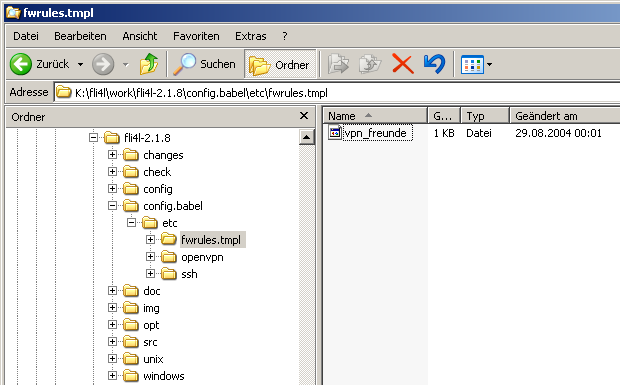
\includegraphics[width=0.9\columnwidth]{etc_fwrules_tmpl_dir}
  \caption{Structure du répertoire fli4l}
  \label{fig:etc_fwrules_tmpl_dir}
\end{figure}

Il est possible de créer vos propre fichier de modèle ou d'utiliser le fichier
existant pour ajouter vos règles. Pour créer votre propre modèle vous devez
simplement créer un fichier avec un nom de modèle que vous voulez et enregistrer
les règles correspondants selon vos besoins. Si vous avez décidé de créer un
fichier modèle, vous devez copier le fichier dans le sous-répertoire
\verb+etc/fwrules.tmpl+ qui sera dans le répertoire \texttt{config}, comme
indiqué dans la figure \ref{fig:etc_fwrules_tmpl_dir}. Si le sous-répertoire
\texttt{etc/fwrules.tmpl} dans le répertoire \texttt{config} n'existe pas,
vous devez créer ce sous-répertoire. les développeurs de paquetages ou les
utilisateurs qui souhaitent créer leurs règles pour plusieurs configurations,
peuvent stocker directement le fichier modèle dans le répertoire
\texttt{opt/etc/fwrules.tmpl}. Dans ce répertoire, sont enregistré que les
nouveaux fichiers modèles. Dans le répertoire \texttt{config} les fichiers
modèles pour les règles sont prioritères au répertoire utilisateur. Enfin, vous
pouvez copier le fichier modèle original fourni par fli4l qui est déjà
\flqq{}configuré\frqq{}, puis coller le contenu dans votre propre fichier,vous
pouvez ensuite enregistrer dans le répertoire \texttt{config}.

Par exemple, si vous voulez ajouter le modèle \fwmatch{vpn\_freunde} vous devez
d'abord créer le fichier \texttt{vpn\_freunde}. Ensuite vous devez enregistrer
les services suivants, \protocol{ssh}, \protocol{smtp}, \protocol{dns} et
\protocol{samba}. Le fichier \texttt{vpn\_freunde} doit ressembler à ceci~:

\begin{example}
\begin{verbatim}
    prot:tcp 22
    prot:tcp 25
    53
    prot:udp 137-138
    prot:tcp 139
    prot:tcp 445
\end{verbatim}
\end{example}

\noindent Maintenant à chaque fois que vous utilisez le modèle \fwmatch{vpn\_freunde}
des règles que vous avez enregistrez seront génèrées pour tous les protocoles
et les ports spécifiés. Exemple avec une action \verb+PF\_FORWARD\_x='tmpl:vpn\_freunde ACCEPT'+,
les règles du \fwchain{FORWARD} seront les suivantes~:

\begin{example}
\begin{verbatim}
    prot:tcp 22 ACCEPT
    prot:tcp 25 ACCEPT
    53 ACCEPT
    prot:udp 137-138 ACCEPT
    prot:tcp 139 ACCEPT
    prot:tcp 445 ACCEPT
\end{verbatim}
\end{example}

\subsection{Configuration du filtrage de paquets}

Le filtrage de paquets est configurable essentiellement par cinq chaînes
voir le tableau~:

\begin{itemize}
  \item \var{PF\_INPUT\_\%} se configure avec la chaîne \fwchain{INPUT},
  \item \var{PF\_FORWARD\_\%} se configure avec la chaîne \fwchain{FORWARD},
  \item \var{PF\_OUTPUT\_\%} se configure avec la chaîne \fwchain{OUTPUT},
  \item \var{PF\_PREROUTING\_\%} se configure avec la chaîne \fwchain{PREROUTING} et
  \item \var{PF\_POSTROUTING\_\%} se configure avec la chaîne \fwchain{POSTROUTING}.
\end{itemize}

Dans la variable \configlabel{PF\_LOG\_LEVEL}{PFLOGLEVEL} on régle le niveau
de journalisation, valable pour l'ensemble les variables, voici les valeurs que
l'on peut paramètrer~: \fwloglevel{debug}, \fwloglevel{info}, \fwloglevel{notice},
\fwloglevel{warning}, \fwloglevel{err}, \fwloglevel{crit}, \fwloglevel{alert},
\fwloglevel{emerg}.

\subsubsection{Chaîne \fwchain{INPUT}}

Configuration de la chaîne \fwchain{INPUT}, c'est ici que les paquets entre
dans le routeur, les hôtes peuvent interroger le routeur. S'il n'y a pas de
règle définie, pour la chaîne \fwchain{INPUT} l'action par défaut sera déterminée,
que faut il faire du paquet lorsqu'il est refusé, la variable de protocole
détermine si le paquet doit être écrit dans le journal du système.

Il y a deux restrictions, au sujet des paramètres à utilisés~:
\begin{itemize}
  \item Seul les valeurs \fwaction{ACCEPT}, \fwaction{DROP} et \fwaction{REJECT}
    sont spécifiés comme action.
  \item Lors d'une restriction d'interface vous ne pouvez que restreindre
    l'interface d'entrée.
\end{itemize}

\begin{description}
\config{PF\_INPUT\_POLICY}{PF\_INPUT\_POLICY}{PFINPUTPOLICY}
Cette variable décrit l'action par défaut, qui est utilisé lorsque aucune autre
règle ne s'applique. Les options sont~:

\begin{itemize}
\item \fwaction{ACCEPT} (pas recommandé)
\item \fwaction{REJECT}
\item \fwaction{DROP} (pas recommandé)
\end{itemize}

\config{PF\_INPUT\_ACCEPT\_DEF}{PF\_INPUT\_ACCEPT\_DEF}{PFINPUTACCEPTDEF}
Si cette variable est sur 'yes', les règles par défaut sont générées, cela est
nécessaires pour un bon fonctionnement du routeur. vous devez indiquer 'yes' pour
une configuration par défaut.

Si vous avez besoin de définir le comportement du routeur, vous devez indiquer
'no'. Vous devez alors paramétrer toutes les règles vous-mêmes. Un comportement
par défaut pour une configuration équivalente devrait ressembler à ceci,
(la description des chaînes définies par l'utilisateur est \jump{sec:userlists}{ici})~:

\begin{example}
{\footnotesize
\begin{verbatim}
    PF_INPUT_ACCEPT_DEF='no'
    #
    # limit ICMP echo requests - use a separate chain
    #
    PF_USR_CHAIN_N='1'
    PF_USR_CHAIN_1_NAME='usr-in-icmp'
    PF_USR_CHAIN_1_RULE_N='2'
    PF_USR_CHAIN_1_RULE_1='prot:icmp:echo-request length:0-150 limit:1/second:5 ACCEPT'
    PF_USR_CHAIN_1_RULE_2='state:RELATED ACCEPT'

    PF_INPUT_N='4'
    PF_INPUT_1='prot:icmp usr-in-icmp'
    PF_INPUT_2='state:ESTABLISHED,RELATED ACCEPT'
    PF_INPUT_3='if:lo:any ACCEPT'
    PF_INPUT_4='state:NEW 127.0.0.1 DROP BIDIRECTIONAL'
\end{verbatim}}
\end{example}

La première règle limite le contrôle des erreurs avec la chaîne "usr-in-icmp".
La deuxième règle accepte seulement les paquets qui appartiennent à une connexion
existante (c. à d. que les paquets sont dans un état \fwpktstate{ESTABLISHED}
ou \fwpktstate{RELATED}), la troisième règle permet la communication locale
avec (\verb+if:lo:any ACCEPT+). La quatrième règle filtre les paquets qui
prétendent avoir une communication locale, mais qui n'ont pas été acceptées
par la règle précédente.

Si vous travaillez avec OpenVPN, vous devez ajouter des
règles, l'utilisation de ces paquets comportent les chaînes suivante~:

\begin{example}
\begin{verbatim}
    PF_INPUT_N='5'
    ...
    PF_INPUT_5='ovpn-chain'
\end{verbatim}
\end{example}

\config{PF\_INPUT\_LOG}{PF\_INPUT\_LOG}{PFINPUTLOG}
Ici on définit, si les paquets refusés doivent être enregistrés par le Kernel.
Pour recevoir les messages vous devez activez la variable \var{OPT\_KLOGD}
via le démon syslog, les messages reçus sont fonction de votre configuration.

\config{PF\_INPUT\_LOG\_LIMIT}{PF\_INPUT\_LOG\_LIMIT}{PFINPUTLOGLIMIT}
Vous définissez dans cette variable la fréquence les entrées générée dans le
journal. La fréquence pour la limites de restriction est décrite de façon
analogue comme ceci \emph{n/Unité de temps} avec un Burst (ou en rafale).
Par exemple \texttt{3/minute:5}. Si la valeur par défaut est vide, la valeur
\texttt{1/second:5} sera utilisé. Si vous indiquez \texttt{none} aucune limite
ne sera effectuée.

\configlabel{PF\_INPUT\_UDP\_REJ\_LIMIT}{PFINPUTUDPREJLIMIT}
\config{PF\_INPUT\_REJ\_LIMIT PF\_INPUT\_UDP\_REJ\_LIMIT}{PF\_INPUT\_REJ\_LIMIT}{PFINPUTREJLIMIT}
Ici on définit la fréquence de refus du paquet entrant, le paquet générée sera
\fwaction{REJECT}. La fréquence de la limite de restriction est décrite de
façon analogue comme ceci \emph{n/Unité de temps} avec un Burst (ou en rafale)
par exemple \texttt{3/minute:5}. Lorsque la limite est dépassée, le paquet sera
simplement ignoré (\fwaction{DROP}). Si la valeur par défaut est vide, la valeur
\texttt{1/second:5} sera utilisé. Si vous indiquez \texttt{none} aucune limite
ne sera effectuée.

\config{PF\_INPUT\_ICMP\_ECHO\_REQ\_LIMIT}{PF\_INPUT\_ICMP\_ECHO\_REQ\_LIMIT}{PFINPUTICMPECHOREQLIMIT}
Ici on définit la fréquence de comment répondre à une demande echo ICMP. La
fréquence de la limite de restriction est décrite de façon analogue comme ceci
\emph{n/Unité de temps} avec un Burst (ou en rafale) par exemple \texttt{3/minute:5}.
Lorsque la limite est dépassée, le paquet sera simplement ignoré (\fwaction{DROP}).
Si la valeur par défaut est vide, la valeur \texttt{1/second:5} sera utilisé.
Si vous indiquez \texttt{none} aucune limite ne sera effectuée.

\config{PF\_INPUT\_ICMP\_ECHO\_REQ\_SIZE}{PF\_INPUT\_ICMP\_ECHO\_REQ\_SIZE}{PFINPUTICMPECHOREQSIZE}
Vous définissez dans cette variable la taille d'une demande d'écho ICMP reçu en
(en octets). Ce chiffre vient s'ajouter à la charge de "l'en-tête" du paquet,
cela est à pendre en considération. La valeur par défaut est de 150 octets.

\configlabel{PF\_INPUT\_x}{PFINPUTx}
\configlabel{PF\_INPUT\_x\_COMMENT}{PFINPUTxCOMMENT}
\config{PF\_INPUT\_N PF\_INPUT\_x PF\_INPUT\_x\_COMMENT}{PF\_INPUT\_N}{PFINPUTN}
Vous indiquez dans cette liste de règles, les paquets qui sont acceptés ou
rejetés par le routeur.
\end{description}

\subsubsection{Chaîne \fwchain{FORWARD}}

Configuration de la chaîne \fwchain{FORWARD}, c'est ici que le routeur
redirige les paquets. S'il n'y a pas de règle définie, pour la chaîne
\fwchain{FORWARD} l'action par défaut sera déterminée, que faut il faire du
paquet lorsqu'il est refusé, la variable de protocole détermine si le paquet
doit être écrit dans le journal du système.

Les paramètres utilisés pour les actions de restriction sont, \fwaction{ACCEPT},
\fwaction{DROP} et \fwaction{REJECT}

\begin{description}
\config{PF\_FORWARD\_POLICY}{PF\_FORWARD\_POLICY}{PFFORWARDPOLICY}
Cette variable décrit l'action par défaut qui sera utilisée, lorsque aucune
autre règle ne s'applique. Les options sont~:

\begin{itemize}
\item \fwaction{ACCEPT}
\item \fwaction{REJECT}
\item \fwaction{DROP}
\end{itemize}

\config{PF\_FORWARD\_ACCEPT\_DEF}{PF\_FORWARD\_ACCEPT\_DEF}{PFFORWARDACCEPTDEF}
Ici on détermine si le routeur accepte les paquets appartenant à des connexions
existantes. Si cette variable est paramétrée sur 'yes', fli4l génère automatiquement
la règle qui accepte les paquets dans un état approprié~:

\verb+'state:ESTABLISHED,RELATED ACCEPT'+,

poursuite de la règle, rejette des paquets avec l'état inconnu~:

\verb+'state:INVALID DROP'+.

et enfin la règle ignore les paquets avec une adresse IP usurpée~:

\verb+'state:NEW 127.0.0.1 DROP BIDIRECTIONAL'+.

En outre, d'autres sous-systèmes générent les règles par défaut~-- Voici une
configuration sans les règles par défaut, avec la redirection de port et
l'OpenVPN la configuration devrait contenir au moins les règles suivantes~:

\begin{example}
\begin{verbatim}
    PF_FORWARD_ACCEPT_DEF='no'
    PF_FORWARD_N='5'
    PF_FORWARD_1='state:ESTABLISHED,RELATED ACCEPT'
    PF_FORWARD_2='state:INVALID DROP'
    PF_FORWARD_3='state:NEW 127.0.0.1 DROP BIDIRECTIONAL'
    PF_FORWARD_4='pfwaccess-chain'
    PF_FORWARD_5='ovpn-chain'
\end{verbatim}
\end{example}

\config{PF\_FORWARD\_LOG}{PF\_FORWARD\_LOG}{PFFORWARDLOG}
Ici on définit, si les paquets refusés doivent être enregistrés par le Kernel.
Pour recevoir les messages vous devez activez la variable \var{OPT\_KLOGD}
via le démon syslog, les messages reçus sont fonction de votre configuration.

\config{PF\_FORWARD\_LOG\_LIMIT}{PF\_FORWARD\_LOG\_LIMIT}{PFFORWARDLOGLIMIT}
Vous définissez dans cette variable la fréquence les entrées générée dans le
journal. La fréquence pour la limites de restriction est décrite de façon
analogue comme ceci \emph{n/Unité de temps} avec un Burst (ou en rafale).
Par exemple \texttt{3/minute:5}. Si la valeur par défaut est vide, la valeur
\texttt{1/second:5} sera utilisé. Si vous indiquez \texttt{none} aucune limite
ne sera effectuée.

\configlabel{PF\_FORWARD\_UDP\_REJ\_LIMIT}{PFFORWARDUDPREJLIMIT}
\config{PF\_FORWARD\_REJ\_LIMIT PF\_FORWARD\_UDP\_REJ\_LIMIT}{PF\_FORWARD\_REJ\_LIMIT}{PFFORWARDREJLIMIT}
Ici on définit la fréquence de refus du paquet entrant, le paquet générée sera
\fwaction{REJECT}. La fréquence de la limite de restriction est décrite de
façon analogue comme ceci \emph{n/Unité de temps} avec un Burst (ou en rafale)
par exemple \texttt{3/minute:5}. Lorsque la limite est dépassée, le paquet sera
simplement ignoré (\fwaction{DROP}). Si la valeur par défaut est vide, la valeur
\texttt{1/second:5} sera utilisé. Si vous indiquez \texttt{none} aucune limite
ne sera effectuée.

\configlabel{PF\_FORWARD\_x}{PFFORWARDx}
\configlabel{PF\_FORWARD\_x\_COMMENT}{PFFORWARDxCOMMENT}
\config{PF\_FORWARD\_N PF\_FORWARD\_x PF\_FORWARD\_x\_COMMENT}{PF\_FORWARD\_N}{PFFORWARDN}
Vous indiquez dans cette liste de règles, les paquets qui sont redirigés
ou rejetés par le routeur.
\end{description}

\subsubsection{Chaîne \fwchain{OUTPUT}}

Configuration de la La chaîne \fwchain{OUTPUT}, c'est ici que le routeur gére
ces paquets sortant. S'il n'y a pas de règle définie, pour la chaîne
\fwchain{OUTPUT} l'action par défaut sera déterminée, que faut il faire du
paquet lorsqu'il est refusé, la variable de protocole détermine si le paquet
doit être écrit dans le journal du système.

Les paramètres utilisés pour les actions de restriction sont~:
\begin{itemize}
  \item Vous devez utilisé seulement les actions \fwaction{ACCEPT}, \fwaction{DROP}
    et \fwaction{REJECT}.
  \item Lors d'une restriction d'interface, la chaîne ne peut que restreindre
  l'interface de sortie.
\end{itemize}

\begin{description}
\config{PF\_OUTPUT\_POLICY}{PF\_OUTPUT\_POLICY}{PFOUTPUTPOLICY}
Cette variable décrit l'action par défaut qui sera utilisée, lorsque aucune
autre règle ne s'applique. Les options sont~:

\begin{itemize}
\item \fwaction{ACCEPT}
\item \fwaction{REJECT}
\item \fwaction{DROP}
\end{itemize}

\config{PF\_OUTPUT\_ACCEPT\_DEF}{PF\_OUTPUT\_ACCEPT\_DEF}{PFOUTPUTACCEPTDEF}
Si cette variable est sur 'yes', les règles par défaut sont générées, cela est
nécessaires pour un bon fonctionnement du routeur. vous devez indiquer 'yes' pour
une configuration par défaut.

Si vous avez besoin de définir le comportement du routeur, vous devez indiquer
'no'. Vous devez alors paramétrer toutes les règles vous-mêmes.Un comportement
par défaut pour une configuration équivalente devrait ressembler à ceci~:

\begin{example}
{\footnotesize
\begin{verbatim}
    PF_OUTPUT_ACCEPT_DEF='no'

    PF_OUTPUT_N='1'
    PF_OUTPUT_1='state:ESTABLISHED,RELATED ACCEPT'
\end{verbatim}}
\end{example}

La première règle (et la seule) accepte seulement les paquets qui appartiennent
à une connexion existante (c'est à dire les paquets qui ont soit l'état
\fwpktstate{ESTABLISHED} ou \fwpktstate{RELATED})

\config{PF\_OUTPUT\_LOG}{PF\_OUTPUT\_LOG}{PFOUTPUTLOG}
Ici on définit, si les paquets refusés doivent être enregistrés par le Kernel.
Pour recevoir les messages vous devez activez la variable \var{OPT\_KLOGD}
via le démon syslog, les messages reçus sont fonction de votre configuration.

\config{PF\_OUTPUT\_LOG\_LIMIT}{PF\_OUTPUT\_LOG\_LIMIT}{PFOUTPUTLOGLIMIT}
Vous définissez dans cette variable la fréquence les entrées générée dans le
journal. La fréquence pour la limites de restriction est décrite de façon
analogue comme ceci \emph{n/Unité de temps} avec un Burst (ou en rafale).
Par exemple \texttt{3/minute:5}. Si la valeur par défaut est vide, la valeur
\texttt{1/second:5} sera utilisé. Si vous indiquez \texttt{none} aucune limite
ne sera effectuée.

\configlabel{PF\_OUTPUT\_UDP\_REJ\_LIMIT}{PFOUTPUTUDPREJLIMIT}
\config{PF\_OUTPUT\_REJ\_LIMIT PF\_OUTPUT\_UDP\_REJ\_LIMIT}{PF\_OUTPUT\_REJ\_LIMIT}{PFOUTPUTREJLIMIT}
Ici on définit la fréquence de refus du paquet entrant, le paquet générée sera
\fwaction{REJECT}. La fréquence de la limite de restriction est décrite de
façon analogue comme ceci \emph{n/Unité de temps} avec un Burst (ou en rafale)
par exemple \texttt{3/minute:5}. Lorsque la limite est dépassée, le paquet sera
simplement ignoré (\fwaction{DROP}). Si la valeur par défaut est vide, la valeur
\texttt{1/second:5} sera utilisé. Si vous indiquez \texttt{none} aucune limite
ne sera effectuée.

\configlabel{PF\_OUTPUT\_x}{PFOUTPUTx}
\configlabel{PF\_OUTPUT\_x\_COMMENT}{PFOUTPUTxCOMMENT}
\config{PF\_OUTPUT\_N PF\_OUTPUT\_x PF\_OUTPUT\_x\_COMMENT}{PF\_OUTPUT\_N}{PFOUTPUTN}
Vous indiquez dans cette liste de règles, les paquets qui sont envoyer
ou rejetés par le routeur.
\end{description}

\marklabel{sec:userlists}{\subsubsection{Chaîne personnalisée}}

Parfois pour différentes raisons, on a besoin d'élaborer nos propres chaînes
pour régler plus précisément le filtrage de paquets. Ces chaînes peuvent
être définies et paramétrées en utilisant la variable \var{PF\_USR\_CHAIN\_\%}.
Les noms de chaîne doivent commencer obligatoirement par \emph{usr-} suivi de
se que vous voulez, ils peuvent être utilisées n'importe ou dans les chaînes
\fwchain{INPUT} ou \fwchain{FORWARD} pour spécifier une action. Par exemple,
voici utilisation de la chaîne de filtrage ICMP~:

\begin{example}
{\footnotesize
\begin{verbatim}
    PF_USR_CHAIN_N='1'
    #
    # create usr-in-icmp
    #
    PF_USR_CHAIN_1_NAME='usr-in-icmp'
    #
    # add rule to usr-in-icmp
    #
    PF_USR_CHAIN_1_RULE_N='2'
    PF_USR_CHAIN_1_RULE_1='prot:icmp:echo-request length:0-150 limit:1/second:5 ACCEPT'
    PF_USR_CHAIN_1_RULE_2='state:RELATED ACCEPT'
    #
    # use chain in PF_INPUT
    #
    PF_INPUT_2='prot:icmp usr-in-icmp'
\end{verbatim}}
\end{example}

\begin{description}
\config{PF\_USR\_CHAIN\_N}{PF\_USR\_CHAIN\_N}{PFUSRCHAINN} Dans cette variable
vous indiquez le nombre de chaîne définie par l'utilisateur.

\config{PF\_USR\_CHAIN\_x\_NAME}{PF\_USR\_CHAIN\_x\_NAME}{PFUSRCHAINxNAME}
Dans cette variable vous indiquez le nom de la chaîne. Le nom doit commencer par
\emph{usr-}.

\configlabel{PF\_USR\_CHAIN\_x\_RULE\_x}{PFUSRCHAINxRULEx}
\configlabel{PF\_USR\_CHAIN\_x\_RULE\_x\_COMMENT}{PFUSRCHAINxRULExCOMMENT}
\config{PF\_USR\_CHAIN\_x\_RULE\_N}{PF\_USR\_CHAIN\_x\_RULE\_N}{dummy0}
\config{PF\_USR\_CHAIN\_x\_RULE\_x}{PF\_USR\_CHAIN\_x\_RULE\_N}{dummy1}
\config{PF\_USR\_CHAIN\_x\_RULE\_x\_COMMENT}{PF\_USR\_CHAIN\_x\_RULE\_N}{PFUSRCHAINxRULEN}
Vous indiquez dans cette liste de règles, les règles définies par l'utilisateur.
Les règles doivent être insérées dans la chaîne \fwchain{FORWARD}. Si aucune
règle ne s'applique le processus sort de la chaîne USR, remonte à la chaîne 
d'origine et continue sur la règle suivante.
\end{description}

\subsubsection{Chaîne NAT (Network Address Translation)}

Les paquets peuvent être manipulés, avant et après les décisions de routage
pour le moment. Par exemple, vous pouvez obtenir une nouvelle adresse de
destination pour la transmission à un autre ordinateur (port forwarding) ou
recevoir une adresse source différente pour masquer le réseau situé derrière
le routeur. Le masquage est utilisé par exemple, pour faire un réseau
privé avec une adresse IP publique ou de cacher une configuration DMZ du
réseau local à partir d'un ordinateur de la DMZ.

La configuration se fait sur deux chaînes, la \fwchain{PREROUTING} et la
\fwchain{POSTROUTING}. Au sujet de la chaînes \fwchain{POSTROUTING} on configure,
les paquets qui seront masqués par le routeur. Si aucune des règles de chaînes
\fwchain{POSTROUTING} ne s'applique, les paquets seront acheminés démasqué.

Pour le masquage, il existe deux versions~: une pour l'interface réseau qui est
assignée lors de la connexion une seule adresse IP (\fwaction{MASQUERADE}) et
une pour l'interface réseau qui utilise une adresse IP statique(\fwaction{SNAT}).
Si vous utilisez \fwaction{SNAT} l'adresse IP doit être enregistrée dans le
paquet source. Les données peuvent être comme ceci.

\begin{itemize}
\item Adresse IP (exemple~: \fwaction{SNAT:1.2.3.4}),
\item Plage d'adresses IP (exemple~: \fwaction{SNAT:1.2.3.4-1.2.3.10})
\item ou comme une référence symbolique (exemple~: \fwaction{SNAT:IP\_NET\_1\_IPADDR})
\end{itemize}

Vous pouvez indiquer un port ou une plage de ports dans \fwaction{SNAT} et aussi
dans \fwaction{MASQUERADE} pour mapper les ports (ou établir une correspondance
entre les ports). Normalement ce n'est pas nécessaire car seul le Kernel peut
sélectionner les ports pour établir une correspondance. Cependant il y a des
applications qui nécessitent que le port source reste inchangé (et imposent un
NAT 1:1 ou elles interdisent le PAT (Port Address Translation) ou NAPT
(Network Address and Port Translation)). La plage de ports est simplement ajouté
après l'adresse IP, par exemple~: \fwaction{SNAT:IP\_NET\_1\_IPADDR:4000-8000}.

La chaînes \fwchain{POSTROUTING} peut utiliser les actions suivantes
\fwaction{ACCEPT}, \fwaction{SNAT}, \fwaction{NETMAP} et \fwaction{MASQUERADE}.

\begin{description}

\configlabel{PF\_POSTROUTING\_x}{PFPOSTROUTINGx}
\configlabel{PF\_POSTROUTING\_x\_COMMENT}{PFPOSTROUTINGxCOMMENT}
\config{PF\_POSTROUTING\_N PF\_POSTROUTING\_x PF\_POSTROUTING\_x\_COMMENT}{PF\_POSTROUTING\_N}{PFPOSTROUTINGN}
\mbox{}\newline
Vous indiquez dans cette liste de règles, des paquets qui seront masquées par 
le routeur (ou transmis non masqué). Si vous ne voulez pas masquer les paquets
qui arrive sur le routeur, vous pouvez placer la règle Accept à la place de
la règle Masquerade.

\end{description}

Dans la chaîne \fwchain{PREROUTING} on configure les paquets qui doivent être
transmis à un autre ordinateur. Si aucune règles de la chaîne \fwchain{PREROUTING}
ne s'applique, les paquets seront ensuite traités sans être changés. L'action
\fwaction{DNAT} attend une adresse IP qui doit être enregistré dans le paquet
en tant que cible. Les données peuvent être comme ceci.

\begin{itemize}
\item Adresse IP (exemple~: \fwaction{DNAT:1.2.3.4}),
\item Plage d'adresses IP (exemple~: \fwaction{DNAT:1.2.3.4-1.2.3.10})
\item Ou comme un nom d'hôte (exemple~: \fwaction{DNAT:@client1})
\end{itemize}

Vous pouvez indiquer un port ou une plage de ports, le port de destination
sera mappée. Cela est nécessaire que si le port doit être changé. Le port est
simplement ajouté après l'adresse IP, par exemple~: \fwaction{DNAT:@server:21}.

L'action \fwaction{REDIRECT} se comporte comme l'action \fwaction{DNAT}, sauf
que l'adresse IP de destination est toujours une adresse IP (primaire) - c'est
l'adresse de l'interface qui est configurée et sur laquelle le paquet arrive,
le paquet sera ensuite livré localement. Cela est nécessaire par exemple
pour un proxy transparent, voir \jump{OPTTRANSPROXY}{\var{OPT\_TRANSPROXY}}.

Si vous voulez faire de la redirection de port sur des interfaces qui utilise
une adresse IP dynamique, pendant le démarrage on ne connaît pas l'adresse IP
du PC vers lesquel les paquets seront dirigés. on peut utiliser la chaîne
\fwchain{PREROUTING} avec le paramètre \fwmatch{dynamic} comme espace réservé
pour assignée l'adresse IP plus tard. Par exemple~:

\begin{example}
{\footnotesize
\begin{verbatim}
    'dynamic:80  DNAT:1.2.3.4'           # rediriger les paquets http vers
                                         # l'adresse IP 1.2.3.4
    'prot:gre any dynamic DNAT:1.2.3.4'  # rediriger les paquets gre (fait partie
                                         # du protocole PPTP) vers l'adresse
                                         # 1.2.3.4 
\end{verbatim}}
\end{example}

La chaînes \fwchain{PREROUTING} peut utiliser les actions suivantes
\fwaction{ACCEPT}, \fwaction{DNAT}, \fwaction{NETMAP} et \fwaction{REDIRECT}.

Pour d'autres exemples sur la façon d faire de la redirection de port,
voir la paragraphe suivant.

\begin{description}
\configlabel{PF\_PREROUTING\_x}{PFPREROUTINGx}
\configlabel{PF\_PREROUTING\_x\_COMMENT}{PFPREROUTINGxCOMMENT}
\config{PF\_PREROUTING\_N PF\_PREROUTING\_x PF\_PREROUTING\_x\_COMMENT}{PF\_PREROUTING\_N}{PFPREROUTINGN}
\mbox{}\newline
Vous indiquez dans cette liste de règles, les paquets transmis par le routeur
vers une cible différente.
\end{description}

\subsection{Exemples}

Voici quelques exemples de configuration du filtrage de paquets.

\subsubsection{Configuration par défaut de fli4l}

Ci-dessous la configuration par défaut de la chaîne \fwchain{INPUT}, cela
nous permet d'atteindre la distribution fli4l~:

\begin{example}
\begin{verbatim}
    PF_INPUT_POLICY='REJECT'
    PF_INPUT_ACCEPT_DEF='yes'
    PF_INPUT_LOG='no'
    PF_INPUT_N='1'
    PF_INPUT_1='IP_NET_1 ACCEPT'
\end{verbatim}
\end{example}

Ainsi, nous obtenons, une
\begin{itemize}
\item autoration pour l'accés au routeur des ordinateurs du réseau local
  (\verb+PF_INPUT_1='IP_NET_1 ACCEPT'+),
\item la communication local est autorisé sur le routeur
  (\verb+PF_INPUT_ACCEPT_DEF='yes'+),
\item les paquets appartenant à une connexions établies par le routeur seront
  acceptées \newline (\verb+PF_INPUT_ACCEPT_DEF='yes'+),
\item tout le reste est rejeté (\verb+PF_INPUT_POLICY='REJECT'+),
\item rien ne sera écrit dans le journal du système
  (\verb+PF_INPUT_LOG='no'+).
\end{itemize}

Pour la chaîne \fwchain{FORWARD} voici la configuration~: seuls les paquets
sur le réseau local et les paquets correspondant à une connexions établies par
les ordinateurs du réseau local doivent être transmis. En outre, les paquets
NetBIOS et CIFS seront rejetés.

\begin{example}
\begin{verbatim}
    PF_FORWARD_POLICY='REJECT'
    PF_FORWARD_ACCEPT_DEF='yes'
    PF_FORWARD_LOG='no'
    PF_FORWARD_N='2'
    PF_FORWARD_1='tmpl:samba DROP'
    PF_FORWARD_2='IP_NET_1 ACCEPT'
\end{verbatim}
\end{example}

Ce que l'on voit ici, est la dépendance de l'ordre des règles~: en \emph{premier}
on rejette les paquets Netbios et \emph{ensuite} les paquets du réseau local
sont acceptés.

Maintenant, le réseau local communique avec le routeur, les paquets sont
transmis, il ne manque que le masquage, il est nécessaire pour accéder au
réseau privé sur Internet~:

\begin{example}
\begin{verbatim}
    PF_POSTROUTING_N='1'
    PF_POSTROUTING_1='IP_NET_1 MASQUERADE'
\end{verbatim}
\end{example}

\subsubsection{Trusted Nets}

Si vous voulez mettre en place plusieurs sous-réseaux locaux qui puissent
communiquer les uns avec les autres librement et sans être masqués, nous devons
nous assurer que les paquets ne seront pas rejetés entre ces sous-réseaux et
qu'ils ne soient pas masqués. Pour cela il suffit de rajouter une règle ou
modifier l'existante.

Supposons que nous ayons un accès DSL via PPPoE, avec deux sous-réseaux
\var{IP\_NET\_1} (192.168.6.0/24) et \var{IP\_NET\_2} (192.168.7.0/24).
La configuration ressemblerait alors à ce qui suit~:

\begin{example}
\begin{verbatim}
    PF_FORWARD_POLICY='REJECT'
    PF_FORWARD_ACCEPT_DEF='yes'
    PF_FORWARD_LOG='no'
    PF_FORWARD_N='4'
    PF_FORWARD_1='IP_NET_1 IP_NET_2 ACCEPT BIDIRECTIONAL'
    PF_FORWARD_2='tmpl:samba DROP'
    PF_FORWARD_3='IP_NET_1 ACCEPT'
    PF_FORWARD_4='IP_NET_2 ACCEPT'

    PF_POSTROUTING_N='3'
    PF_POSTROUTING_1='IP_NET_1 IP_NET_2 ACCEPT BIDIRECTIONAL'
    PF_POSTROUTING_2='IP_NET_1 MASQUERADE'
    PF_POSTROUTING_3='IP_NET_2 MASQUERADE'
\end{verbatim}
\end{example}

Maintenant, les règles occupent les paquets qui sont acheminés entre les deux
sous-réseaux sans examen plus approfondi. La troisième et quatrième règles
font en sorte que les deux sous-réseaux sont disponible pour aller sur
Internet. La première règle de la chaîne \fwchain{POSTROUTING} assure que
la communication entre les sous-réseaux se fait démasqué.

Alternativement, on peut dire que seuls les paquets qui dépassent par
l'interface \fwmatch{pppoe} doivent être masqués~:

\begin{example}
\begin{verbatim}
    PF_POSTROUTING_N='1'
    PF_POSTROUTING_1='if:any:pppoe MASQUERADE'
\end{verbatim}
\end{example}

De même, on pourrait limiter le filtrage des ports sur l'interface \fwmatch{pppoe}
et les deux sous-réseaux peuvent être combinés en un seul, voici la configuration~:

\begin{example}
\begin{verbatim}
    PF_FORWARD_POLICY='REJECT'
    PF_FORWARD_ACCEPT_DEF='yes'
    PF_FORWARD_LOG='no'
    PF_FORWARD_N='2'
    PF_FORWARD_1='if:any:pppoe tmpl:samba DROP'
    PF_FORWARD_2='192.168.6.0/23 ACCEPT'

    PF_POSTROUTING_N='1'
    PF_POSTROUTING_1='if:any:pppoe MASQUERADE'
\end{verbatim}
\end{example}

Les paquets qui passent par l'interface \fwmatch{pppoe}, qui sont adressée
au \protocol{udp} Ports 137-138 ou au \protocol{tcp} Ports 139 et 445 seront
rejeté (règle~1), tous les autres paquets qui viennent du sous-réseau 
192.168.6.0/23, sont transmis (la règle~2).

\subsubsection{Route Network}

Si vous voulez ajouter le réseau 10.0.0.0/24 dans le réseau existant (par ex.
pour avoir un accès à distance sur ce réseau), de plus si vous voulez
communiquer en étant démasqué et rejeter les paquets des \protocol{udp}
Ports 137-138 et aussi des\protocol{tcp} Ports 139 et 445, la configuration
se présentera comme ceci~:

\begin{example}
\begin{verbatim}
    PF_FORWARD_POLICY='REJECT'
    PF_FORWARD_ACCEPT_DEF='yes'
    PF_FORWARD_LOG='no'
    PF_FORWARD_N='4'
    PF_FORWARD_1='IP_NET_1 IP_NET_2 ACCEPT BIDIRECTIONAL'
    PF_FORWARD_2='tmpl:samba DROP'
    PF_FORWARD_3='192.168.6.0/23 ACCEPT'
    PF_FORWARD_4='10.0.0.0/24 ACCEPT'

    PF_POSTROUTING_N='2'
    PF_POSTROUTING_1='10.0.0.0/24 ACCEPT BIDIRECTIONAL'
    PF_POSTROUTING_2='192.168.6.0/23 MASQUERADE'
\end{verbatim}
\end{example}

\begin{itemize}
\item Règle~1 permet une communication claire entre les sous-réseaux
  \var{IP\_NET\_1} et \var{IP\_NET\_2}.
\item Règle~2 rejette les paquets pour les ports samba.
\item Règle~3 et 4 permet la transmission de paquets provenant des sous-réseaux
  192.168.6.0/24, 192.168.7.0/24 und 10.0.0.0/24, dans l'autre direction cela
  c'est déjà inclus dans le paramètre \verb+PF_FORWARD_ACCEPT_DEF='yes'+
\item Règle~1 la chaîne \fwchain{POSTROUTING} garantit que les paquets ne sont
pas masquées dans ou sur le sous-réseau 10.0.0.0/24
\end{itemize}

Une alternative à la configuration précédante~:

\begin{example}
\begin{verbatim}
    PF_POSTROUTING_N='1'
    PF_POSTROUTING_1='if:any:pppoe MASQUERADE'
\end{verbatim}
\end{example}

Dans cette règle seul les paquets qui dépassent par l'interface \fwmatch{pppoe}
doivent être masqués.

\subsubsection{Liste noir, liste blanche}

Listes noires (ou blacklists) (on refuse aux ordinateurs de cette liste
"de faire quelque chose") et liste blanches (ou Whitelists) (on permet aux
ordinateurs de cette liste "de faire quelque chose") la mis en place est en
principe semblable. Les règles écritent au début de la liste sont très
spécifiques et sont plus générique vers la fin de la liste. Dans une liste noir
les règles au début de la liste seront interdit de faite quoi que se soit et
en fin de liste ils pourront fait quelque chose. Avec une liste blanche, c'est
tout le contraire.

\emph{Exemple~1~:} tous les ordinateurs du sous-réseau 192.168.6.0/24 peuvent
accéder à Internet sauf l'ordinateur 12, ils ne pourront pas communiquer
avec le protocole CIFS par les ports 137-138 (\protocol{udp}), 139 et 445
(\protocol{tcp})

\begin{example}
\begin{verbatim}
    PF_FORWARD_POLICY='REJECT'
    PF_FORWARD_ACCEPT_DEF='yes'
    PF_FORWARD_LOG='no'
    PF_FORWARD_N='3'
    PF_FORWARD_1='192.168.6.12 DROP'
    PF_FORWARD_2='tmpl:samba DROP'
    PF_FORWARD_3='192.168.6.0/23 ACCEPT'

    PF_POSTROUTING_N='1'
    PF_POSTROUTING_2='192.168.6.0/24 MASQUERADE'
\end{verbatim}
\end{example}

\emph{Exemple~2~:} l'ordinateur 12 peut accéder à Internet (mais on interdit
toujours les Ports \ldots), tous les sous-réseaux locaux peuvent communiquer
entre eux.

\begin{example}
\begin{verbatim}
    PF_FORWARD_POLICY='REJECT'
    PF_FORWARD_ACCEPT_DEF='yes'
    PF_FORWARD_LOG='no'
    PF_FORWARD_N='3'
    PF_FORWARD_1='192.168.6.0/24 192.168.7.0/24 ACCEPT BIDIRECTIONAL'
    PF_FORWARD_2='tmpl:samba DROP'
    PF_FORWARD_3='192.168.6.12 ACCEPT'

    PF_POSTROUTING_N='1'
    PF_POSTROUTING_1='if:any:pppoe MASQUERADE'
\end{verbatim}
\end{example}

\subsection{Configuration par défaut}

\subsubsection{Simple routeur masquant un réseau derrière lui}

\begin{example}
\begin{verbatim}
#
# Accès au routeur
#
PF_INPUT_POLICY='REJECT'
PF_INPUT_ACCEPT_DEF='yes'
PF_INPUT_LOG='no'
PF_INPUT_N='1'
PF_INPUT_1='IP_NET_1 ACCEPT'   # Tous les hôtes du réseau local
                               # peuvent communiquer avec le routeur

#
# Accés à "Internet"
#
PF_FORWARD_POLICY='REJECT'
PF_FORWARD_ACCEPT_DEF='yes'
PF_FORWARD_LOG='no'

PF_FORWARD_N='2'
PF_FORWARD_1='tmpl:samba DROP' # Les paquets samba qui veulent
                               # sortir du réseau sont rejetés
PF_FORWARD_2='IP_NET_1 ACCEPT' # Tous les paquets du réseau local
                               # peuvent sortir

#
# Masquage du réseau local
#
PF_POSTROUTING_N='1'
PF_POSTROUTING_1='IP_NET_1 MASQUERADE'  # Masque des paquets qui quittent
                                        # le sous-réseau
\end{verbatim}
\end{example}

\subsubsection{Simple routeur masquant deux réseaux derrière lui}

\begin{example}
\begin{verbatim}
#
# Accès au routeur
#
PF_INPUT_POLICY='REJECT'
PF_INPUT_ACCEPT_DEF='yes'
PF_INPUT_LOG='no'
PF_INPUT_N='2'
PF_INPUT_1='IP_NET_1 ACCEPT'   # Tous les hôtes du réseau local
                               # peuvent communiquer avec le routeur
PF_INPUT_2='IP_NET_2 ACCEPT'   # Tous les hôtes du réseau local
                               # peuvent communiquer avec le routeur

#
# Accés à "Internet"
#
PF_FORWARD_POLICY='REJECT'
PF_FORWARD_ACCEPT_DEF='yes'
PF_FORWARD_LOG='no'

#
# Libre communication entre les réseaux
#
PF_FORWARD_N='4'
PF_FORWARD_1='IP_NET_1 IP_NET_2 ACCEPT BIDIRECTIONAL'
PF_FORWARD_2='tmpl:samba DROP' # Les paquets samba qui veulent
                               # sortir du réseau sont rejetés
PF_FORWARD_3='IP_NET_1 ACCEPT' # Tous les paquets du réseau local
                               # peuvent sortir
PF_FORWARD_4='IP_NET_2 ACCEPT' # Tous les paquets du réseau local
                               # peuvent sortir

#
# Masquage des réseaux locaux, la communication entre les réseaux
# ne sont pas masquées
#
PF_POSTROUTING_N='3'
PF_POSTROUTING_1'IP_NET_1 IP_NET_2 ACCEPT BIDIRECTIONAL'
PF_POSTROUTING_2='IP_NET_1 MASQUERADE'  # les paquets quittent le sous-réseau
                                        # masqués
PF_POSTROUTING_3='IP_NET_2 MASQUERADE'  # les paquets quittent le sous-réseau
                                        # masqués
\end{verbatim}
\end{example}

\subsubsection{Masquage de deux réseaux derrière le routeur DSL
avec un accés SSH/HTTP par Internet}

\begin{example}
\begin{verbatim}
#
# Accès au routeur
#
PF_INPUT_POLICY='REJECT'
PF_INPUT_ACCEPT_DEF='yes'
PF_INPUT_LOG='no'
PF_INPUT_N='4'
PF_INPUT_1='IP_NET_1 ACCEPT'   # Tous les hôtes du réseau local
                               # peuvent communiquer avec le routeur
PF_INPUT_2='IP_NET_2 ACCEPT'   # Tous les hôtes du réseau local
                               # peuvent communiquer avec le routeur
PF_INPUT_3='tmpl:ssh ACCEPT'   # Permettre l'accès au service SSH
                               # depuis n'importe où
PF_INPUT_4='tmpl:http 1.2.3.4/24 ACCEPT'   # Permettre aux ordinateurs
                               # du sous-réseau d'avoir un accès
                               # spécifique au service HTTP

#
# Accés à "Internet"
#
PF_FORWARD_POLICY='REJECT'
PF_FORWARD_ACCEPT_DEF='yes'
PF_FORWARD_LOG='no'

#
# Pas de communication entre les réseaux, les deux réseaux peuvent
# avoir accés à Internet, paquets Samba sont rejetés
#
PF_FORWARD_N='2'
PF_FORWARD_1='tmpl:samba if:any:pppoe DROP' # Les paquets samba qui sortent
                               # du réseau sont rejetés
PF_FORWARD_2='if:any:pppoe ACCEPT' # Tous les autres paquets peuvent
                               # quitter le réseau local

#
# Masquage des réseaux locaux, la communication entre les réseaux
# ne sont pas masquées
#
PF_POSTROUTING_N='1'
PF_POSTROUTING_1='if:any:pppoe MASQUERADE'  # Les paquets sont masqués
                                            #en quitter le sous-réseau
\end{verbatim}
\end{example}

\subsubsection{Port Forwarding}

La redirection de port peut être personnalisé avec la chaîne \fwchain{PREROUTING},
vous devez paramétrer la règle de la façon suivante, dans (\verb+TARGET+ vous
indiquez l'adresse IP de destination d'origine (optionnel) et le port de
destination d'origine, dans \verb+NEW_TARGET+ vous indiquez la nouvelle adresse
de destination et le nouveau port de destination (optionnel), dans \verb+PROTOCOL+
vous indiquez le protocole correspondant)~:

\begin{example}
\begin{verbatim}
    TARGET='<port>'
    NEW_TARGET='<ip>'
    PROTOCOL='<proto>'
    PF_PREROUTING_x='prot:<proto> dynamic:<port> DNAT:<ip>'

    TARGET='<port1>-<port2>'
    NEW_TARGET='<ip>'
    PROTOCOL='<proto>'
    PF_PREROUTING_x='prot:<proto> dynamic:<port1>-<port2> DNAT:<ip>'

    TARGET='<ip>:<port-a>'
    NEW_TARGET='<ip>:<port-b>'
    PROTOCOL='<proto>'
    PF_PREROUTING_x='prot:<proto> any <ip>:<port-a> DNAT:<ip>:<port-b>'
\end{verbatim}
\end{example}

\subsubsection{Proxy transparent}

Si vous souhaitez autoriser un accès spécifique à Internet, uniquement via un
proxy local sans que le client s'en aperçoive, vous pouvez utiliser les
chaînes \fwchain{PREROUTING} et \fwchain{POSTROUTING}. Fondamentalement,
trois étapes sont nécessaires~:

\begin{enumerate}
\item Les requêtes qui arrivent sur le port http seront
  détournées sur le proxy (\fwchain{PREROUTING}).
\item Modification des paquets du proxy pour les rediriger, afin que le routeur
  pense que les paquets viennent de lui, si bien qu'il les renvoie à
  nouveau (\fwchain{POSTROUTING}).
\item Les paquets passent à travers la chaîne (\fwchain{PREROUTING})
  s'il n'existe pas de règle dans la chaîne (\fwchain{FORWARD})

\begin{example}
\begin{verbatim}
PF_FORWARD_x='IP_NET_1 ACCEPT'
\end{verbatim}
\end{example}
\end{enumerate}

\emph{Exemple~1~:} supposons que nous ayons un seul réseau \var{IP\_NET\_1},
sur lequel on a installé Squid sur un ordinateur avec le nom \host{proxy} et
que vous voulez router le trafic \protocol{http} sur cette ordinateur. Squid
écoute sur le port 3128. Par souci de simplicité, nous allons nous référer au
nom d'hôte \host{@proxy} enregistré dans \verb+HOST_1_NAME='proxy'+ (voir
\jump{sec:domainkonfiguration}{Domaine de configuration}).

L'ensemble devrait ressembler à ceci~:

\begin{example}
\begin{verbatim}
...
  PF_PREROUTING_x='@proxy ACCEPT'
      # Les paquets du Proxy ne doivent pas être détournés

  PF_PREROUTING_x='prot:tcp IP_NET_1 80 DNAT:@proxy:3128'
      # Les paquets HTTP de IP_NET_1 allant sur n'importe quelle destination
      # seront redirigés vers @proxy, Port 3128

  PF_POSTROUTING_x='any @proxy:3128 SNAT:IP_NET_1_IPADDR'
      # Tous les paquets du Proxy sur le Port du 3128 seront réécrient
      # comme s'ils venaient de fli4l (IP_NET_1_IPADDR)

  PF_FORWARD_x='prot:tcp @proxy 80 ACCEPT'
      # La règle de la chaîne FORWARD laisse passés les paquets HTTP du proxy (si nécessaire)
...
\end{verbatim}
\end{example}

Il peut y avoir plusieurs conflits potentiels avec d'autres réseaux ou de
reditection de port (se n'est rien d'autre qu'une règle \fwaction{DNAT}),
il va falloir formuler encore plus rigoureusement les règles.


\emph{Exemple~2~:} notre Proxy qui s'appel \host{proxy} se trouve dans le réseau
\var{IP\_NET\_1}, il écoute sur le port 3128 et sera efficace uniquement pour
les clients du réseau \var{IP\_NET\_1}. Le réseau \var{IP\_NET\_1} est accessible
via l'interface \var{IP\_NET\_1\_DEV}. Les paquets provenant des autres réseaux
ne seront pas pris en considération.

\begin{example}
\begin{verbatim}
...
  PF_PREROUTING_x='if:IP_NET_1_DEV:any !@proxy 80 DNAT:@proxy:3128'
      # Les demandes vers le port HTTP, ne viennent pas du proxy, mais via
      # l'interface interne (IP_NET_1_DEV) et rediriger vers le port proxy.
      # A ce stade, le contrôle if:IP_NET_1_DEV:any est important pour vérifier
      # si les paquets viennent bien de l'intérieur, autrement les paquets
      # seraient également diriger vers l'extérieur (faille de sécurité~!)

  PF_POSTROUTING_x='prot:tcp IP_NET_1 @proxy:3128 SNAT:IP_NET_1_IPADDR'
      # Les paquets HTTP provenant de IP_NET_1 sont réécrits pour être envoyés
      # sur le port 3128 du proxy, comme s'ils venaient de fli4l (IP_NET_1_IPADDR)

  PF_FORWARD_x='prot:tcp @proxy 80 ACCEPT'
      # La règle de la chaîne FORWARD laisse passer les paquet http du Proxy (si nécessaire)
...
\end{verbatim}
\end{example}

\emph{Exemple~3~:} pour vous rendre la vie plus facile et pour rendre les
règles un peu plus courtes, vous pouvez également utiliser le modèle (voir
\jump{sec:templates}{Modèle pour le filtrage de paquets}). A ce stade
\fwmatch{tmpl:http} est utilisé, il se traduit par \fwmatch{prot:tcp any any:80}.
Par exemple à partir de \fwmatch{tmpl:http IP\_NET\_1 DNAT:@proxy:3128} ou
alors \fwmatch{prot:tcp IP\_NET\_1 80 DNAT:@proxy:3128}.

Les deux réseaux \var{IP\_NET\_1} et \var{IP\_NET\_2} doivent être transparent
sur le Proxy. Cela pourrait vous aider à simplifier l'écriture

\begin{example}
\begin{verbatim}
...
  PF_PREROUTING_x='tmpl:http @proxy ACCEPT'
      # Les paquets http ne doivent pas être détournés

  PF_PREROUTING_x='tmpl:http IP_NET_1 DNAT:@proxy:3128'
      # Les paquets HTTP provenant de IP_NET_1 sont détournés

  PF_PREROUTING_x='tmpl:http IP_NET_2 DNAT:@proxy:3128'
      # Les paquets HTTP provenant de IP_NET_2 sont détournés

  PF_POSTROUTING_x='IP_NET_1 @proxy:3128 SNAT:IP_NET_1_IPADDR'
  PF_POSTROUTING_x='IP_NET_2 @proxy:3128 SNAT:IP_NET_2_IPADDR'

  PF_FORWARD_x='tmpl:http @proxy ACCEPT'
...
\end{verbatim}
\end{example}

Cela peut se poursuivre indéfiniment \ldots

\marklabel{sec:dmz}{\subsection{DMZ~-- Zone démilitarisée}}

fli4l permet également la construction d'une simple DMZ. Tout d'abord, vous
pouvez voir sur le site wiki https://ssl.nettworks.org/wiki un exemple de
configuration.

\marklabel{sec:masqueradingmodule}{\subsection{Conntrack Helpers}}

  Bien que l'utilisation du masquage d'IP \index{Masquerading} a l'avantage
  que plusieurs ordinateurs du réseau local peuvent être acheminés via
  une adresse IP publique, mais il y a aussi des inconvénients que vous devez
  prendre en compte.

  Le gros problème est, par exemple, qu'aucun ordinateur de l'extérieur ne peut
  se connecter à un ordinateur du réseau local. C'est souhaitable pour des
  raisons de sécurité, mais certains protocoles ne fonctionnent pas car ils
  requièrent une connexion depuis l'extérieur.

  Un exemple classique le FTP. En plus du canal de communication, les commandes
  et les réponses sont échangés sur un autre canal (sous la forme d'un port-IP)
  pour envoyer les données. fli4l utilise pour cela Conntrack Helper
  qui permet de transmettre les ports supplémentaires, ils sont utilisés pour
  déverrouiller le ad hoc et aussi pour les ordinateurs internes quand c'est
  nécessaire. Conntrack Helper "écoute" le flux de données afin de détecter
  si un port supplémentaire est nécessaire.

  Les applications typiques pour Conntrack Helper sont le protocole pour le Chat
  et pour les jeux sur Internet.

  Vous activez Conntrack Helper avec des règles et un ensemble de variables
  spécifiques. Dans la liste de règles \var{PF\_PREROUTING\_CT\_\%} les
  affectations contiendra les Helpers pour les paquets venant de l'extérieur,
  dans la liste de règles \var{PF\_OUTPUT\_CT\_\%} les affectations contiendront
  les Helpers pour les paquets générés par le routeur. Quelques exemples
  pratiques viendront illustrer cela.

\emph{Exemple~1~:} si vous voulez autoriser le mode FTP actif sur le réseau
  local, le routeur sera visible à partir de cette connexion par les routeurs
  extérieur, pour cela vous devez créer une règle dans la chaîne
  \var{PF\_PREROUTING\_CT\_\%} comme ceci~:

\begin{example}
\begin{verbatim}
    PF_PREROUTING_CT_N='1'
    PF_PREROUTING_CT_1='tmpl:ftp IP_NET_1 HELPER:ftp'
\end{verbatim}
\end{example}

  pour toutes les connexions TCP depuis le réseau local (\var{IP\_NET\_1}) vers
  toute autre adresse sur le port 21 (c'est le Port du \protocol{ftp}) le module
  auxiliaire \protocol{ftp} est chargé. Ce module permet alors de se connecter,
  le serveur FTP peut établir une connexion vers client pour le transfert de
  données, un "trou" est temporairement ouvert dans le pare-feu.

  \emph{Exemple~2~:} avec le mode FTP passif, il vous permet d'activer un
  serveur FTP sur le réseau local (ainsi une connexion de données sera établie
  vers l'extérieur, là aussi un trou dans le pare-feu sera ouvert), ici le
  routeur sera également visible à partir de cette connexion par les routeurs
  extérieur. La règle est représentée de la manière suivante~:

\begin{example}
\begin{verbatim}
    PF_PREROUTING_CT_N='1'
    PF_PREROUTING_CT_1='tmpl:ftp any dynamic HELPER:ftp'
\end{verbatim}
\end{example}

Cette règle se traduit de la manière suivante, toutes les connexions FTP seront
envoyés à l'adresse dynamique du routeur, associé à Conntrack Helper du FTP. Ici
\fwmatch{dynamic} a été utilisé car il est supposé que le routeur est
responsable de la connexion Internet et a donc une adresse IP externe. Si le
routeur effectue une connexion via DSL, la règle peut aussi s'écrire~:

\begin{example}
\begin{verbatim}
    PF_PREROUTING_CT_N='1'
    PF_PREROUTING_CT_1='tmpl:ftp if:pppoe:any HELPER:ftp'
\end{verbatim}
\end{example}

Cette règle se traduit de la manière suivante, toutes les connexions FTP sur
l'interfase DSL (\fwmatch{pppoe}), seront associées à Conntrack Helper du FTP.

Si le routeur ne se connecte pas, il est par exemple derrière un autre routeur
(box FRITZ!, modem câble, etc), la règle suivante peut être utilisée~:

\begin{example}
\begin{verbatim}
    PF_PREROUTING_CT_N='1'
    PF_PREROUTING_CT_1='tmpl:ftp if:IP_NET_2_DEV:any HELPER:ftp'
\end{verbatim}
\end{example}

  On suppose que dans l'exemple la connexion s'effectue via une interface vers
  l'autre routeur, cette interface est associée au deuxième sous-réseau
  (\var{IP\_NET\_2\_DEV}).

  On notera bien sûr, \emph{en plus} de la configuration il sera nécessaire de
  paramétrer la chaîne \fwchain{FORWARD}, pour réellement faire parvenir les
  paquets FTP. Voici une règle typique~:

  \begin{example}
\begin{verbatim}
    PF_PREROUTING_1='tmpl:ftp any dynamic DNAT:@ftpserver'
\end{verbatim}
\end{example}

   On suppose que l'hôte sur lequel le programme du serveur FTP fonctionne,
   a le nom \host{ftpserver}.

\emph{Exemple~3~:} enfin, le must, si vous souhaitez utiliser le mode FTP actif
  directement à partir de fli4l (avec l'aide du programme \protocol{ftp} qui est
  dans le paquetage \package{tools}). Le pare-feu doit être préparé pour cela,
  cette fois on utilisera la chaîne \fwchain{OUTPUT} et la liste de règles
  \var{PF\_OUTPUT\_CT\_\%} ou l'on va configurer les règles~:

\begin{example}
\begin{verbatim}
    PF_OUTPUT_CT_N='1'
    PF_OUTPUT_CT_1='tmpl:ftp HELPER:ftp'
\end{verbatim}
\end{example}

Cette règle n'est toutefois pas nécessaire si la variable
\verb+FTP_PF_ENABLE_ACTIVE='yes'+ est activée~-- S'il vous plaît reportez-vous
à la documentation du OPT\_protocol{FTP} dans le paquetage \package{tools}

Voici un apperçu de l'actuel Conntrack Helpers~:

\begin{center}
    \begin{longtable}{|l|p{0.5\textwidth}|}
        \hline
        \multicolumn{1}{|l}{\textbf{Helpers}} &
        \multicolumn{1}{|l|}{\textbf{Explication}} \\
        \hline
        \endhead
        \hline
        \endfoot
        \endlastfoot
            \index{ftp}\protocol{ftp}      & File Transfer Protocol\\
        \hline
            \index{h323}\protocol{h323}    & H.323 (Voice over IP)\\
        \hline
            \index{irc}\protocol{irc}      & Internet Relay Chat\\
        \hline
            \index{pptp}\protocol{pptp}    & PPTP Masquerading
                (Ce module peut être plus qu'un client PPTP il fonctionne
                 simultanément derrière un routeur fli4l.)\\
        \hline
            \index{sip}\protocol{sip}      & Session Initiation Protocol\\
        \hline
            \index{sane}\protocol{sane}    & SANE Network Procotol\\
        \hline
            \index{snmp}\protocol{snmp}    & Simple Network Management Protocol\\
        \hline
            \index{tftp}\protocol{tftp}    & Trivial File Transfer Protocol\\
        \hline
        \caption{Disponibilité de Conntrack Helpers dans le filtrage de paquets}\marklabel{fwrule:cthelpers}{}
    \end{longtable}
\end{center}

 Voici un aperçu des variables à configurer~:

\begin{description}
\config{PF\_PREROUTING\_CT\_ACCEPT\_DEF}{PF\_PREROUTING\_CT\_ACCEPT\_DEF}{PFPREROUTINGCTACCEPTDEF}
Si cette variable est sur 'yes', les règles par défaut sont générés, elles
sont nécessaires pour le bon fonctionnement du routeur. Vous devriez
indiquer 'yes' pour l'utilisation par défaut.

\configlabel{PF\_PREROUTING\_CT\_x}{PFPREROUTINGCTx}
\configlabel{PF\_PREROUTING\_CT\_x\_COMMENT}{PFPREROUTINGCTxCOMMENT}
\config{PF\_PREROUTING\_CT\_N PF\_PREROUTING\_CT\_x PF\_PREROUTING\_CT\_x\_COMMENT}{PF\_PREROUTING\_CT\_N}{PFPREROUTINGCTN}
Vous indiquez dans cette liste de règles, les paquets entrants à partir
du routeur seront connectés par Conntrack Helpers.

\config{PF\_OUTPUT\_CT\_ACCEPT\_DEF}{PF\_OUTPUT\_CT\_ACCEPT\_DEF}{PFOUTPUTCTACCEPTDEF}
Si cette variable est sur 'yes', les règles par défaut sont générés, elles
sont nécessaires pour le bon fonctionnement du routeur. Vous devriez
indiquer 'yes' pour l'utilisation par défaut.

\configlabel{PF\_OUTPUT\_CT\_x}{PFOUTPUTCTx}
\configlabel{PF\_OUTPUT\_CT\_x\_COMMENT}{PFOUTPUTCTxCOMMENT}
\config{PF\_OUTPUT\_CT\_N PF\_OUTPUT\_CT\_x PF\_OUTPUT\_CT\_x\_COMMENT}{PF\_OUTPUT\_CT\_N}{PFOUTPUTCTN}
\mbox{}\\
Vous indiquez dans cette liste de règles, les paquets qui sont générés par
le routeur pour une connexion au routeur avec Conntrack Helpers.
\end{description}
